\documentclass{amsart}
\usepackage{amssymb}
\usepackage{tikz}
\usetikzlibrary{calc,automata,positioning,arrows.meta,decorations.markings}
\usepackage{forest}
\usepackage[siunitx]{circuitikz}
\usepackage{pgfplots}
\pgfplotsset{compat=1.18}
\usepackage{tikz-3dplot}
\usepackage{dynkin-diagrams}
\usepackage{spectralsequences}
\usepackage{ytableau}
\begin{document}
%% feature: tikz-basic | lines, circle, filled shape, nodes with math labels
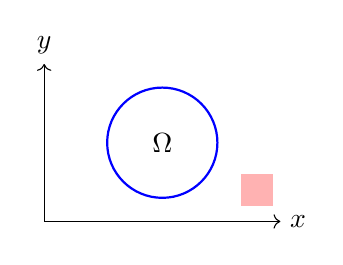
\begin{tikzpicture}
  \draw[->] (0,0) -- (3,0) node[right] {$x$};
  \draw[->] (0,0) -- (0,2) node[above] {$y$};
  \draw[thick, blue] (1.5,1) circle (0.7);
  \fill[red!30] (2.5,0.2) rectangle (2.9,0.6);
  \node at (1.5,1) {$\Omega$};
\end{tikzpicture}
%% feature: tikz-calc | calc coordinates, dashed/dotted, arrow tips, labels on paths
\begin{tikzpicture}
  \coordinate (A) at (0,0); \coordinate (B) at (3,1);
  \draw[dashed] (A) -- (B) node[midway, above, sloped] {$\ell$};
  \draw[dotted, -{Stealth}] (A) -- ($(A)!0.5!(B) + (0,1)$);
  \fill (A) circle (2pt) node[below] {$A$};
  \fill (B) circle (2pt) node[below] {$B$};
\end{tikzpicture}
%% feature: automata | automaton with states, initial/accepting, loop
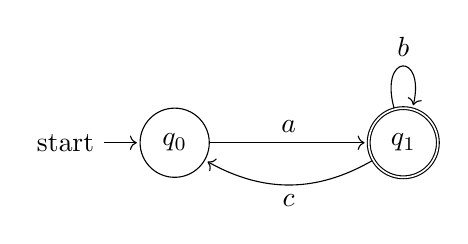
\begin{tikzpicture}[shorten >=1pt, node distance=2cm, auto]
  \node[state, initial] (q0) {$q_0$};
  \node[state, accepting, right=of q0] (q1) {$q_1$};
  \path[->] (q0) edge node {$a$} (q1)
            (q1) edge[loop above] node {$b$} ()
            (q1) edge[bend left] node {$c$} (q0);
\end{tikzpicture}
%% feature: multiline-node | node with explicit line breaks and alignment
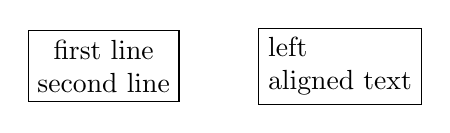
\begin{tikzpicture}
  \node[draw, align=center] (a) {first line\\second line};
  \node[draw, align=left, right=of a] {left\\aligned text};
\end{tikzpicture}
%% feature: forest | forest tree with math nodes
\begin{forest}
  [$S$ [$NP$ [$D$] [$N$]] [$VP$ [$V$] [$NP$]]]
\end{forest}
%% feature: circuitikz | RC circuit with siunitx labels
\begin{circuitikz}
  \draw (0,0) to[V, l=$\SI{5}{\volt}$] (0,2) to[R, l=$R$] (3,2) to[C, l=$C$] (3,0) -- (0,0);
\end{circuitikz}
%% feature: pgfplots | axis with a function plot, domain and legend
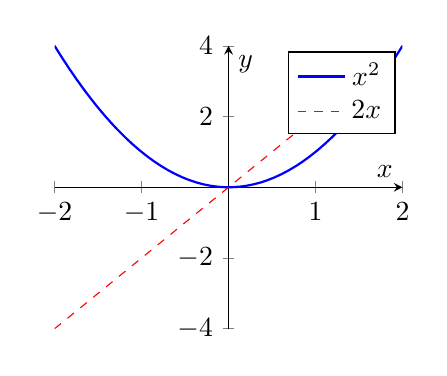
\begin{tikzpicture}
  \begin{axis}[axis lines=middle, xlabel=$x$, ylabel=$y$, domain=-2:2, samples=50, width=6cm]
    \addplot[blue, thick] {x^2};
    \addplot[red, dashed] {2*x};
    \legend{$x^2$, $2x$}
  \end{axis}
\end{tikzpicture}
%% feature: tikz-3dplot | 3D axes with tikz-3dplot rotated coordinates
\tdplotsetmaincoords{70}{110}
\begin{tikzpicture}[tdplot_main_coords]
  \draw[->] (0,0,0) -- (2,0,0) node[anchor=north east] {$x$};
  \draw[->] (0,0,0) -- (0,2,0) node[anchor=north west] {$y$};
  \draw[->] (0,0,0) -- (0,0,2) node[anchor=south] {$z$};
  \draw[blue] (1,1,0) -- (1,1,1.5);
\end{tikzpicture}
%% feature: dynkin | Dynkin diagrams of several types
$\dynkin{A}{4}$ \quad $\dynkin{D}{5}$ \quad $\dynkin{G}{2}$ \quad $\dynkin{E}{8}$
%% feature: sseq | spectral sequence page with classes and a differential
\begin{sseqpage}[classes={draw=none}, homological Serre grading, xscale=1.5]
  \class["\mathbb{Z}"](0,0)
  \class["\mathbb{Z}"](2,0)
  \class["\mathbb{Z}/2"](0,1)
  \d2(2,0)
\end{sseqpage}
%% feature: ytableau | Young diagrams and a filled tableau
$\ydiagram{3,2}$ \quad $\ydiagram{1,1,1}$ \quad
\begin{ytableau} 1 & 2 & 4 \\ 3 & 5 \end{ytableau}
\end{document}
